\chapter {Viziune}

\section{Control}

Găsirea unor noi forme fundamentale de interacțiune cu mediul virtual reprezintă următorul pas atât în evoluția tehnologiei cât și a societății. Apariția realității virtuale și cea augmentată viața publică a atras după sine interesul companiilor și a indivizilor de a utiliza și dezvolta aceste tehnologii, iar obstacolele întâmpinate în acest proces, ca efectul vertigo sau lipsa unor modalități de mișcare naturală încurajează creativitatea și inovația.

Lumea virtuală este la un pas de contopire cu lumea reală, cu companii ca Tesla, Facebook, Google ce au departamente dedicate cercetării și dezvoltării nu doar în domeniul VR/AR dar și al inteligenței artificiale sau neurociberneticii.

Dar nu doar corporații cu rezonanță apar pe lista celor care vor să transforme științifico-fantasticul în realitate, dar și companii mici și mijlocii, cum ar fi enigmatica companie start-up Magic Leap, ce promite introducerea unei tehnologii pe care ei o numesc \textit{mixt reality}, ce va înlocui ecranele standard.

\begin{figure}[h]
  \centering
  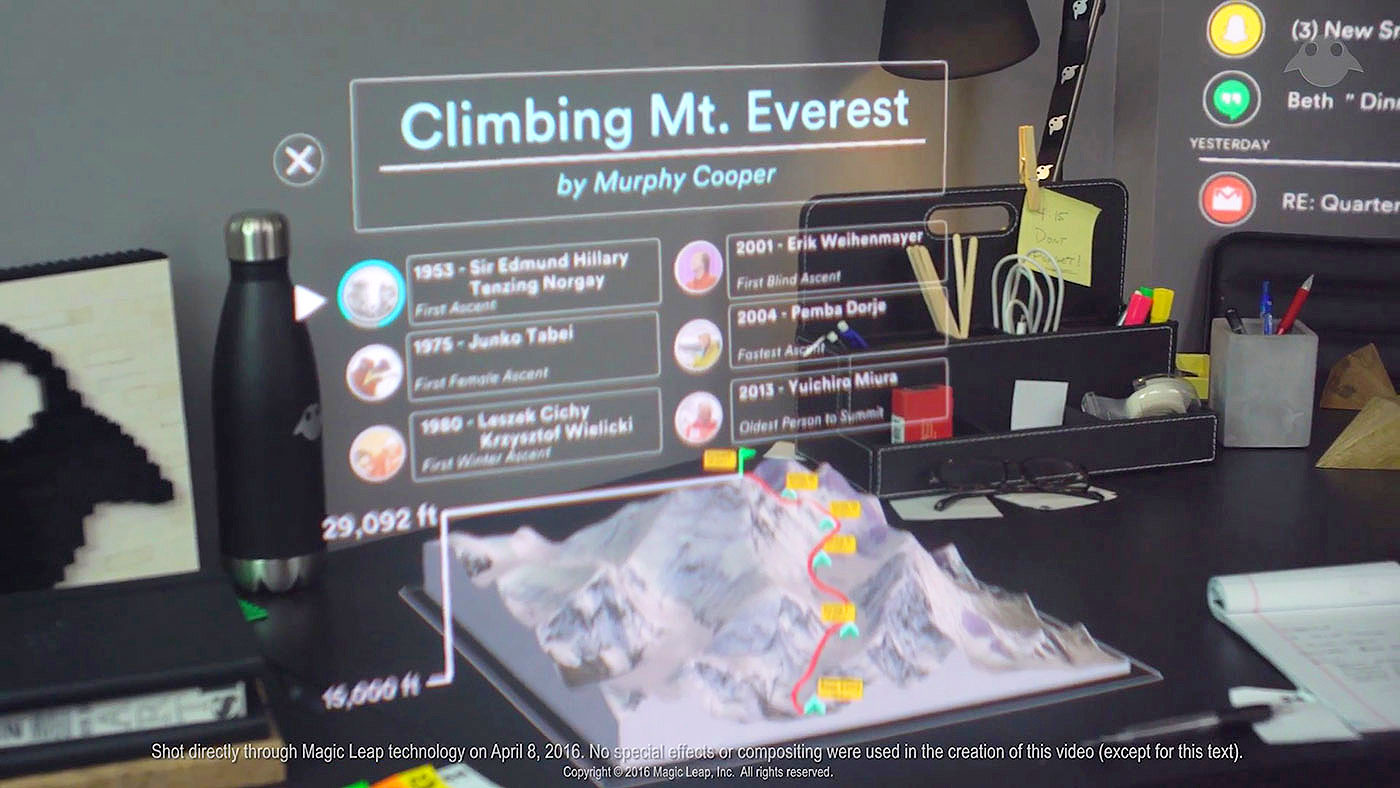
\includegraphics[scale=0.27]{img/magicleap.jpg}
  \caption{Imagine extrasă dintr-un clip demonstrativ distribuit de Magic Leap}
\end{figure}

O altă metodă tot mai populară de a controla aparatura din jurul nostru, este folosirea vocii pentru a vorbi direct cu acestea. Utilizarea comenzilor vocale pentru a interacționa cu telefonu mobil nu este ceva nou, dar gadgeturi ca Amazon Echo, Google Home și mai nou Apple HomePod, cu care putem controla lucruri obișnuite din casă ca becurile, televizorul și termostatul, promovează acest tip de interacțiune și transformă încă un element din universul Star Trek în realitate.

Progrese importante ce ar putea juca un rol extrem de important în viitorul nu foarte îndepărtat au fost făcute și în domeniul neuro-științei. Neurologii reușind să mapeze foarte detaliat cortexul cerebral (scoarța cerebrală), iar computerele devenind suficient de rapide pentru a detecta și interpreta semnalele creierului în timp real, este doar o chestiune de timp până vom putea controla tehnologia direct cu puterea gândului. 

Gândul este proces non-verbal și pur. Este mediul primar prin care ne controlăm corpul iar transformarea creierului  într-un controler direct al tehnologiei reprezintă idealul eficienței de comunicare cu dispozitivele pe care creăm.

Deși pare doar o fantezie această tehnologie deja există.
Compania Emotiv a lansat deja pe piață un astfel de dispozitiv ce poate controla spre exemplu o mașinuță electrică doar prin concentrarea asupra ideii de mișcare.
Dispozitivul este în principiu un mini-electroencefalograf  ce poate detecta undele cerebrale produse când ne concentrăm asupra unui lucru simplu și clar.

\begin{figure}[h]
  \centering
  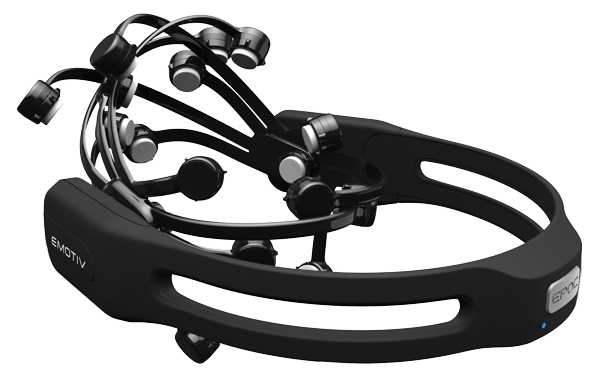
\includegraphics[scale=0.6]{img/emotiv_epoc.png}
  \caption{Dispozitivul Epoc+ dezvoltat de compania Emotiv}
\end{figure}
\newpage

\section{Brain-computer interface}

\textit{Brain-computer interface} prescurtat \textit{BCI}, uneori numit și \textit{mind-machine interface(MMI)} sau \textit{direct neural interface (DNI)} este o cale de comunicare directă între creier și un dispozitiv extern. BCI sunt adesea întrebuințate în cercetarea, maparea, asistarea, augmentarea sau repararea funcțiilor cognitive sau senzoriale ale omului.

Există trei tipuri de BCI:
\begin{itemize}
\item Invazive

\begin{figure}[h]
  \centering
  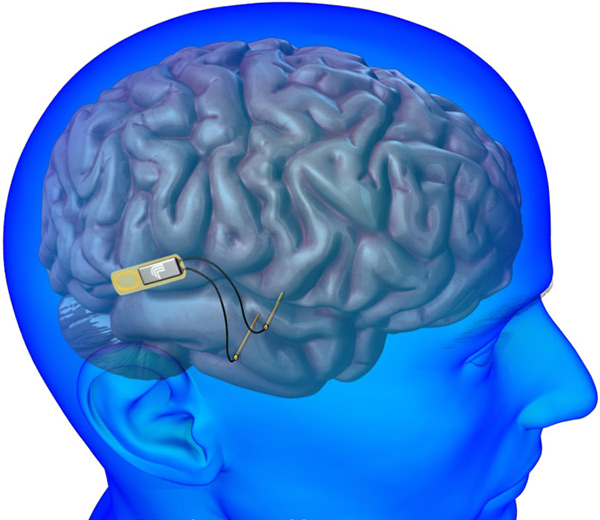
\includegraphics[scale=0.2]{img/invasiveBCI.jpg}
\end{figure}

Dispozitivul de transmitere a semnalelor este implantat direct în materia cenușie. Această metodă produce cea mai înaltă calitate a semnalelor dar acumularea de țesut cicatrizat poate duce la degradarea semnalelor.

\item Parțial invazive

\begin{figure}[h]
  \centering
  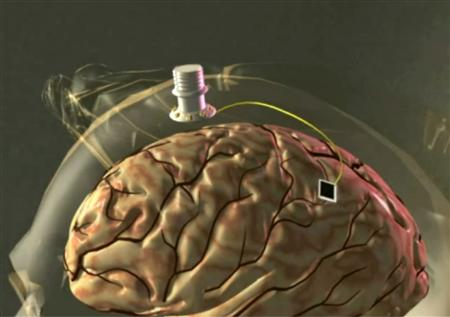
\includegraphics[scale=0.4]{img/BrainGate.jpg}
\end{figure}

Dispozitivul este implantat în interiorul craniului dar nu în țesutul cerebral. Produc semnale de o calitate mai înaltă calitate decât cele non-invazive prin atenuarea efectului inhibitor produs de craniu, și este mai puțin predispus la lezarea țesutului.

\item Non-invazive

\begin{figure}[h]
  \centering
  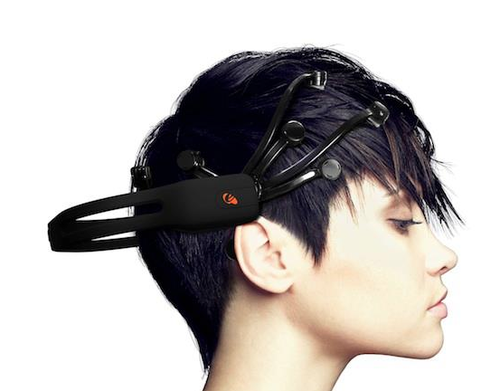
\includegraphics[scale=0.3]{img/noninvasiveBCI.png}
\end{figure}

Implică doar o cască ce înregistrează semnalele electromagnetice transmise de neuroni, fără nevoia niciunui implant. Deși această metodă este cea mai simplă, suferă de rezoluție slabă din cauza interferenței craniului cu semnalele.
\end{itemize}

Aceste tehnologii, în special cele non-intruzive sunt deja disponibile publicului. \textit{OpenBCI} spre exemplu este o companie dedicată să ofere tuturor accesul la date biometrice. Prin intermediul Kickstarter vor să lanseze un dispozitiv BCI open-source.

Alte proiecte ca \textit{Neural Lace}, dezvoltat de noua companie de cercetare medicală lansată de Elon Musk, Neuralink, au ca scop, inițial de a ajuta persoanele cu dizabilități neurologice, iar mai apoi de a augmenta creierul pentru a putea ține pasul cu progresul rapid al inteligenței artificiale.

\section{Singularitate tehnologică}

Singularitatea tehnologică este un concept din futurologie care se referă la implicațiile pe care în general le are progresul tehnico-științific foarte accelerat pentru specia umană și ceea ce înțelegem prin om.

Termenul a fost împrumutat din fizică unde singularitate este de exemplu o gaură neagră, oamenii neputând să afle ce este în interiorul ei, neputând pătrunde dincolo de raza Schwarzschild, legile fizicii nemaiavând valabilitate aici și din  matematică / analiza complexă unde singularitatea este punctul în care o ecuație sau o suprafață degenerează sau dispare.

Extrapolând legea lui Moore, Kurzweil presupune că în cei 100 de ani ai secolului al XXI-lea vom asista la o evoluție comparabilă cu 20.000 de ani precedenți, dacă se menține curba exponențială. Aceasta deoarece odată ce computerele vor depăși performanța creierului uman, ele vor fi capabile să se autoîmbunătățească, menținând ritmul de creștere exponențial al vitezei de calcul. Rezultatul va fi că progresul tehnico-științific va cunoaște o accelerare din ce în ce mai înaltă. Acele computere vor fi în stare până la urmă să descifreze aproape toate secretele naturii și Universului.

Acest presupus salt tehnologic ultrarapid va duce la evenimente aproape imposibil de imaginat pentru specia homo sapiens: contopirea dintre inteligența biologică și cea nebiologică (mind uploading), oameni aproape nemuritori și nivele înalte de superinteligență care se răspândesc rapid în întreg Universul. De aceea este folosit termenul de singularitate: specia umană nu are cum să înțeleagă ce va urma (gaură neagră), la fel cum o bacterie nu poate înțelege ce este un om, atât de mare va fi progresul tehnico-științific.